\message{ !name(paper.tex)}%  article.tex (Version 3.3, released 19 January 2008)
%  Article to demonstrate format for SPIE Proceedings
%  Special instructions are included in this file after the
%  symbol %>>>>
%  Numerous commands are commented out, but included to show how
%  to effect various options, e.g., to print page numbers, etc.
%  This LaTeX source file is composed for LaTeX2e.

%  The following commands have been added in the SPIE class 
%  file (spie.cls) and will not be understood in other classes:
%  \supit{}, \authorinfo{}, \skiplinehalf, \keywords{}
%  The bibliography style file is called spiebib.bst, 
%  which replaces the standard style unstr.bst.  

\documentclass[]{spie}  %>>> use for US letter paper
%%\documentclass[a4paper]{spie}  %>>> use this instead for A4 paper
%%\documentclass[nocompress]{spie}  %>>> to avoid compression of citations
%% \addtolength{\voffset}{9mm}   %>>> moves text field down
%% \renewcommand{\baselinestretch}{1.65}   %>>> 1.65 for double spacing, 1.25 for 1.5 spacing 
%  The following command loads a graphics package to include images 
%  in the document. It may be necessary to specify a DVI driver option,
%  e.g., [dvips], but that may be inappropriate for some LaTeX 
%  installations. 
\usepackage{graphicx}
\usepackage{subfig}
\usepackage{amsmath}
\usepackage{amssymb}
\usepackage{hyperref}

\title{Texture mapping 3D planar models of indoor environments with noisy camera poses} 

%>>>> The author is responsible for formatting the 
%  author list and their institutions.  Use  \skiplinehalf 
%  to separate author list from addresses and between each address.
%  The correspondence between each author and his/her address
%  can be indicated with a superscript in italics, 
%  which is easily obtained with \supit{}.

\author{Peter Cheng, Michael Anderson, Stewart He, Avideh Zakhor
\skiplinehalf
University of California, Berkeley\\
}

 

%%%%%%%%%%%%%%%%%%%%%%%%%%%%%%%%%%%%%%%%%%%%%%%%%%%%%%%%%%%%% 
%>>>> uncomment following for page numbers
% \pagestyle{plain}    
%>>>> uncomment following to start page numbering at 301 
%\setcounter{page}{301} 
 
\begin{document}

\message{ !name(paper.tex) !offset(690) }
\section{Results and Conclusions}
\label{sec:resultsAndConclusions}
Examples of ceilings and floors textured with the tile caching
approach, and walls textured with the shortest path approach, are
displayed in Figure \ref{fig:results}. High resolution texture
comparisons, as well as a walkthrough of a fully textured 3D model are
available in the accompanying video to this paper.

As mentioned earlier, our approach is quite efficient. The top wall in
Figure \ref{fig:results}(a) was generated with 7543 $\times$ 776
pixels, and spans a 40-meter long wall. Given 41000 input images, a
2.8GHz consumer-grade laptop takes approximately a minute to pick 36
candidate images, followed by another minute to perform both image alignment and the shortest
path texturing method, with the majority of computation time spent
calculating SIFT matches within the SiftGPU framework. While not quite
real-time visualization, the process is capable of generating quick
updates after changes in various parameters or modifications to input
data.

In this paper, we have developed two approaches to texture map models
with noisy camera localization data. We are able to refine image
locations based on geometry references and feature matching, and
robustly handle outliers. The tile-based mapping approach can be used
to texture both simple rectangular walls as well as complex floor and
ceiling geometry. We also developed a shortest path texturing method
that produces seamless textures on planes where multiple head-on
images are available. Both of these approaches are highly modular, and
easily tunable for different environments and acquisition systems.

\begin{figure}
  \centering
  \subfloat[][]{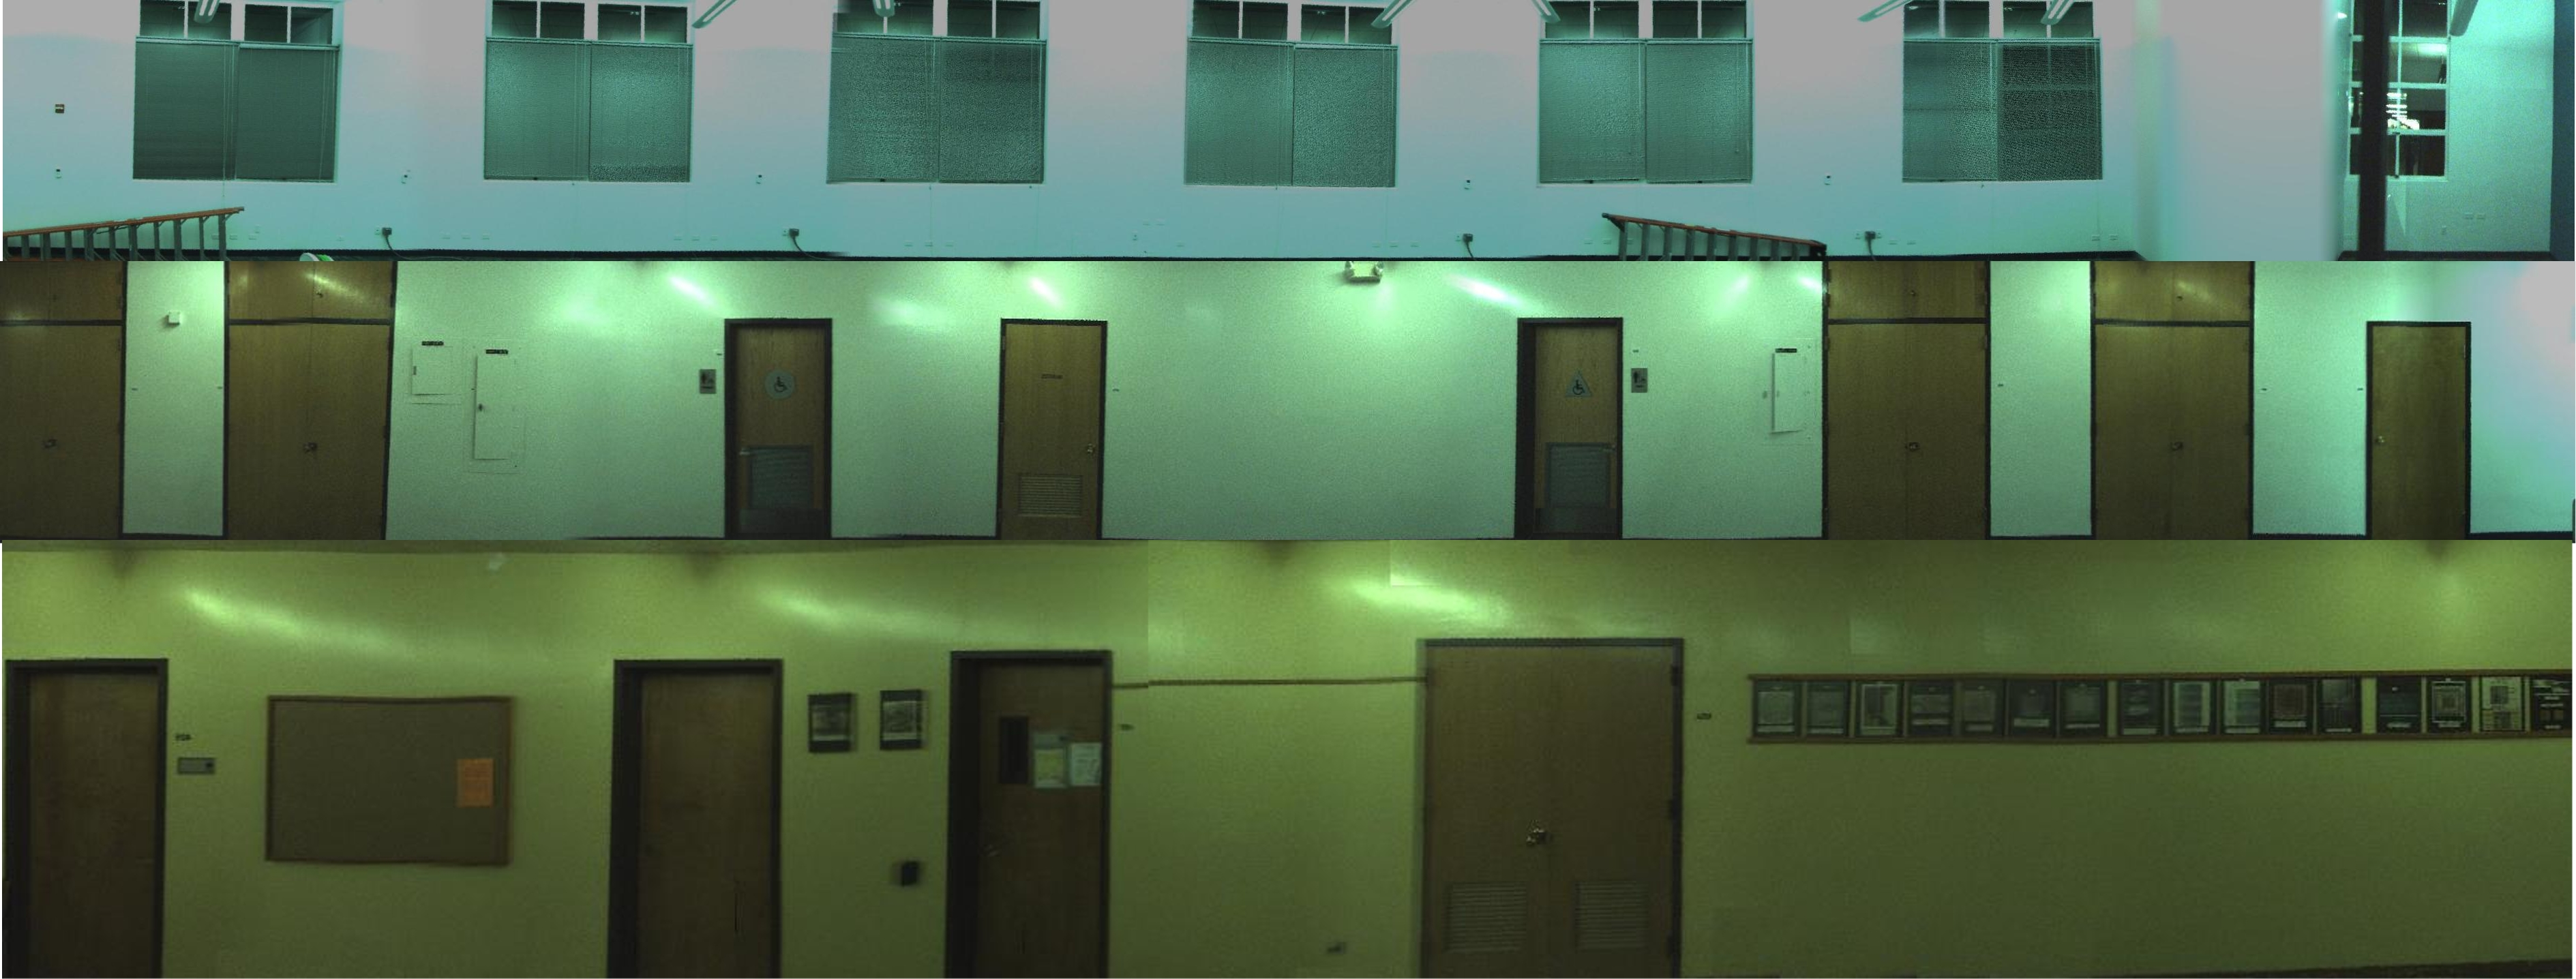
\includegraphics[width=3in]{finalfloors.jpg}} ~~~~~~~~
  \centering
  \subfloat[][]{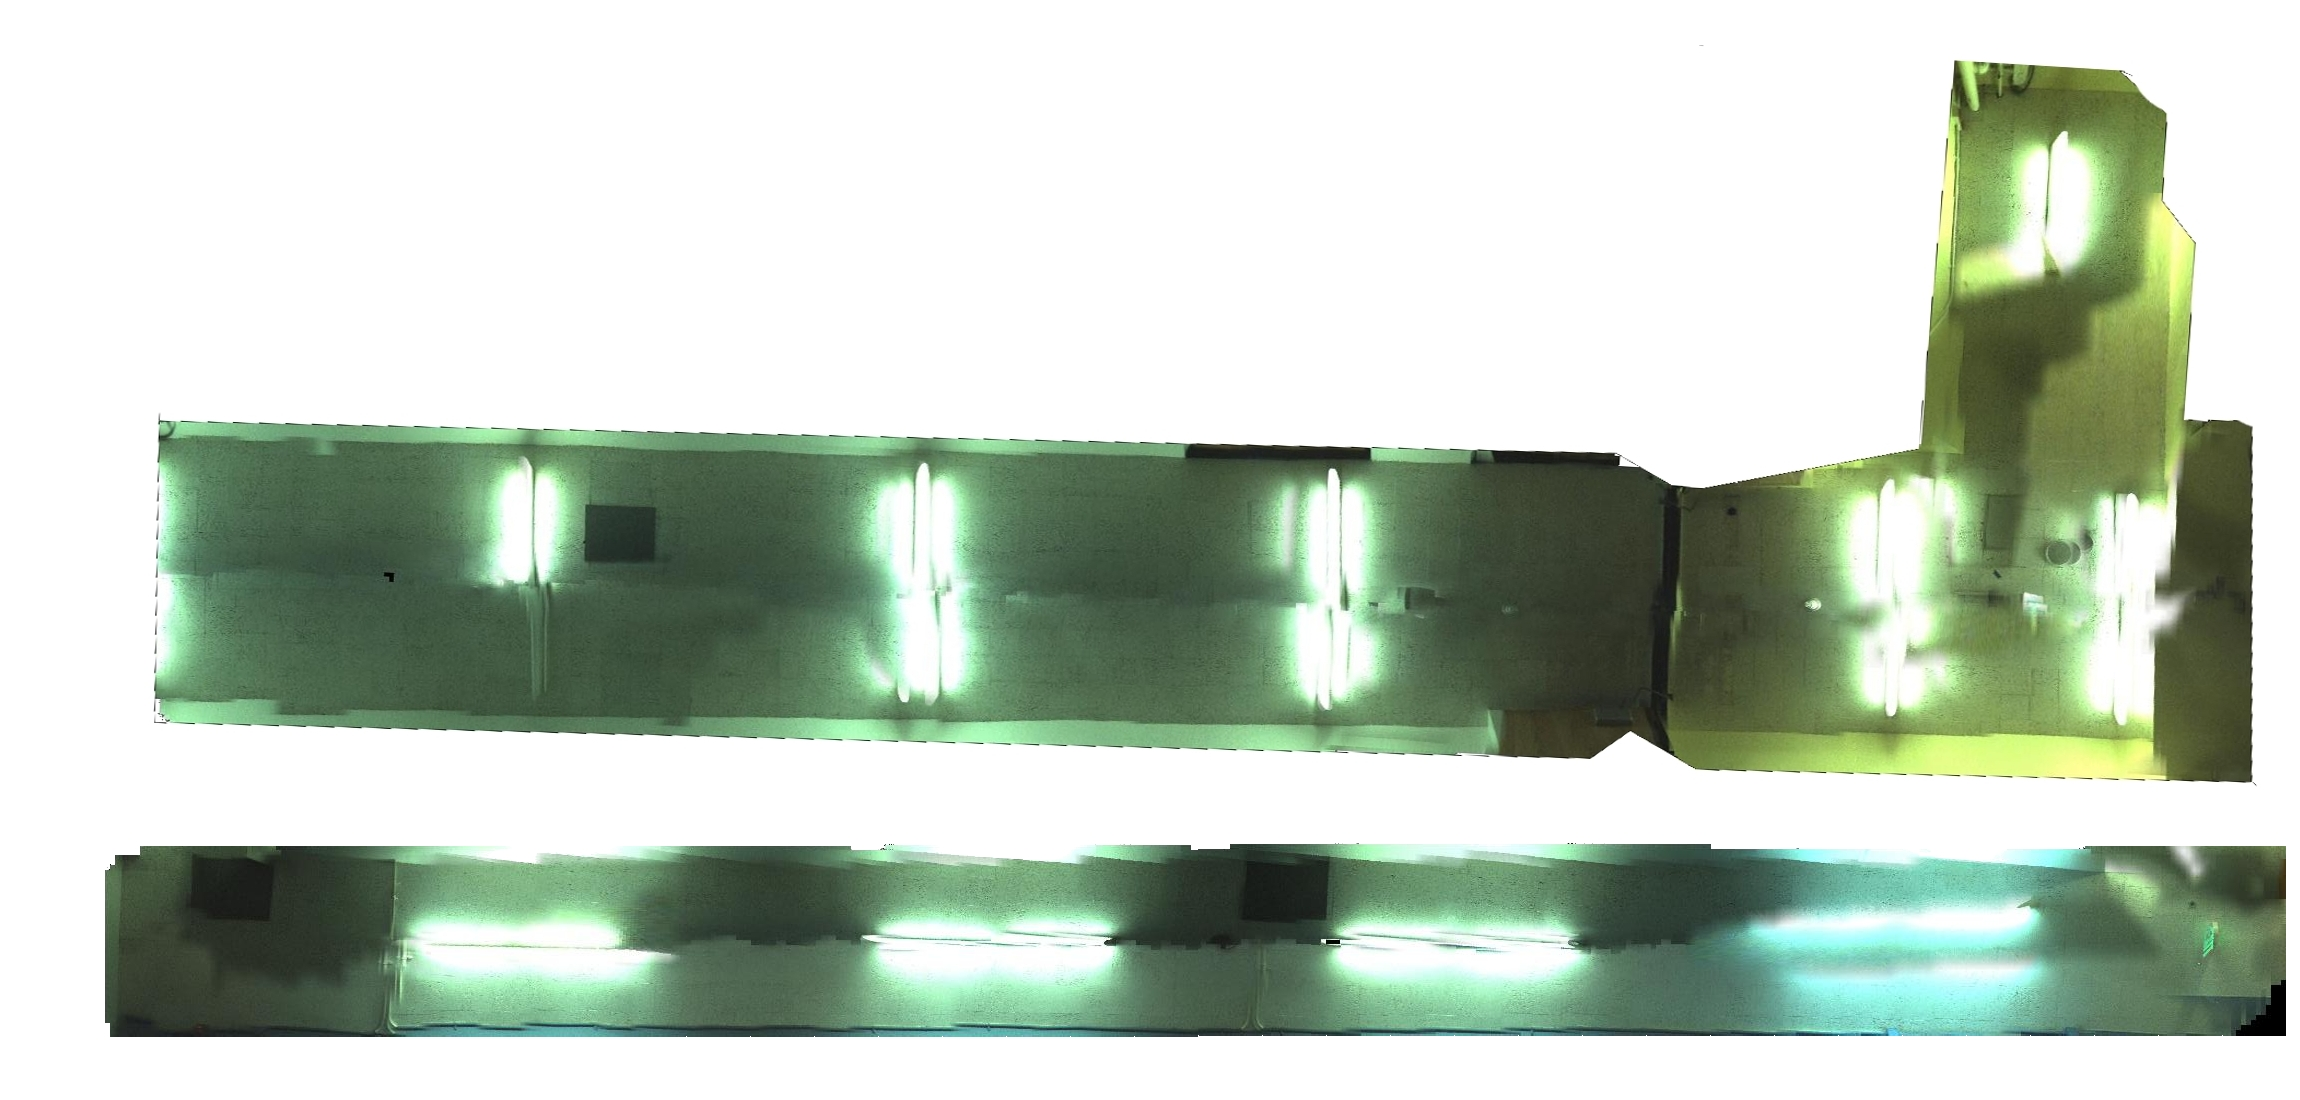
\includegraphics[width=3in]{finalceilings.jpg}}

  \centering \subfloat[][]{
    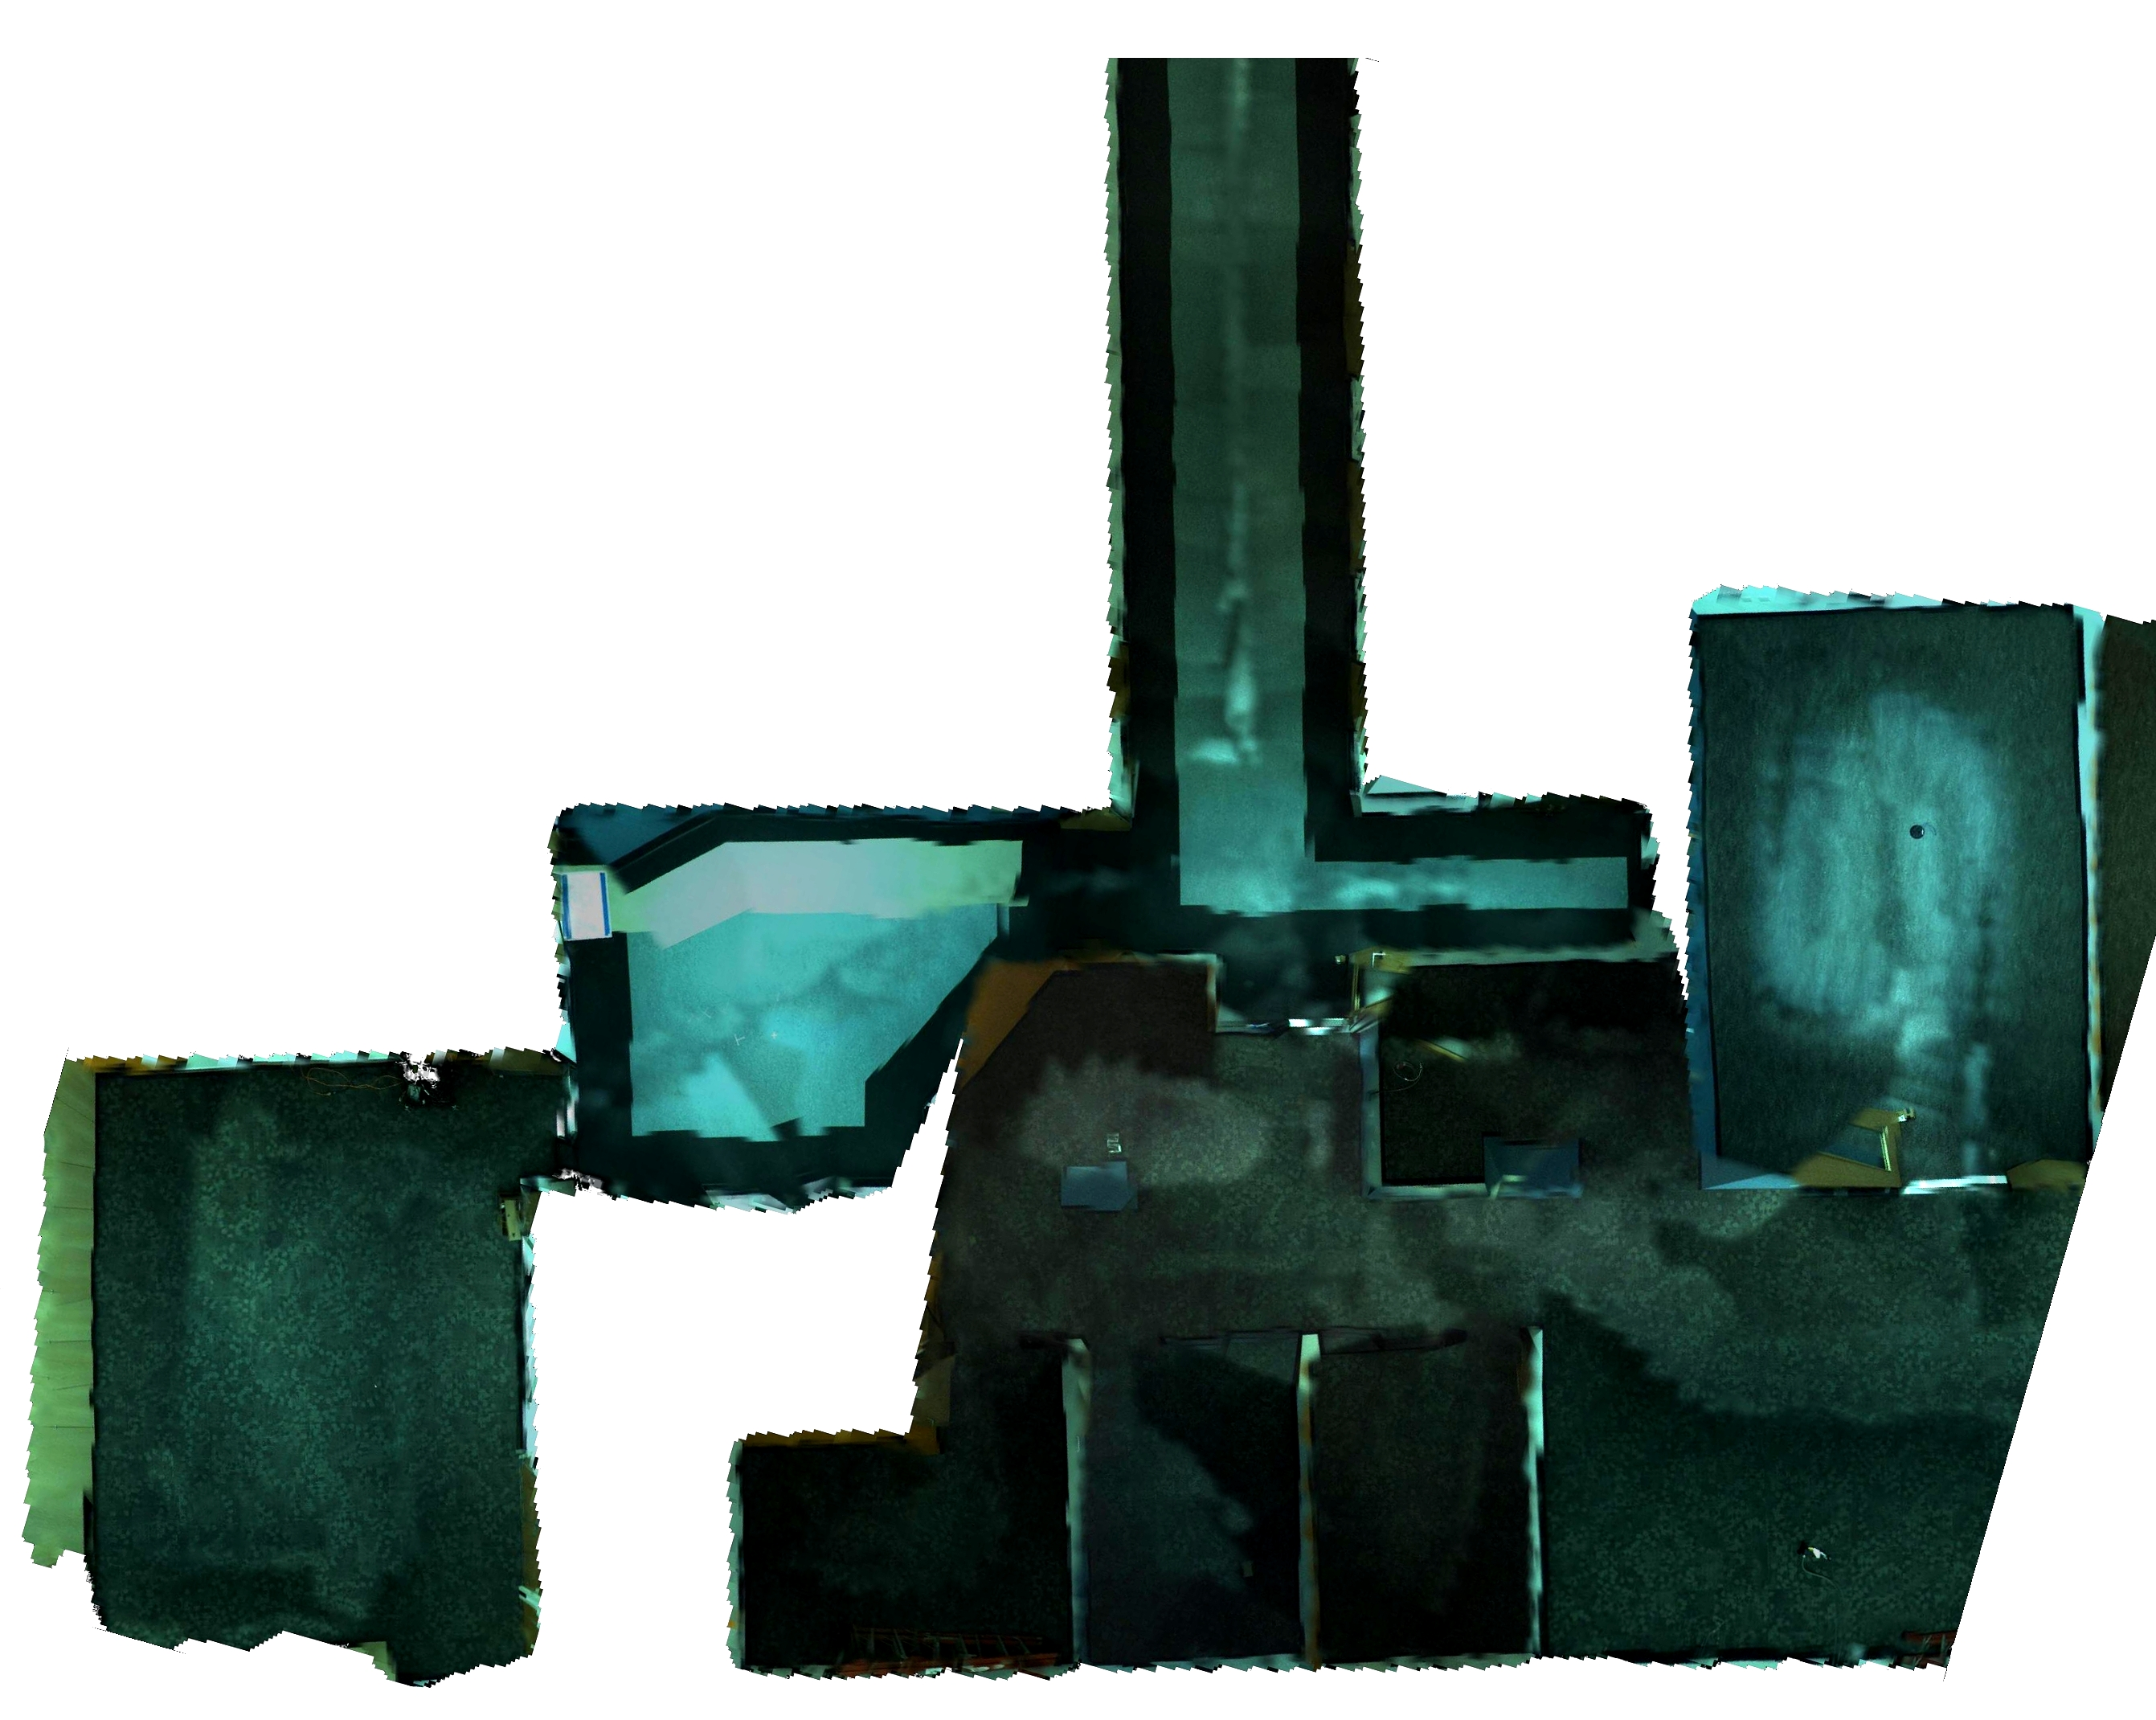
\includegraphics[height=2in, width=3in]{floorcropped.jpg} ~~~~~~~~
    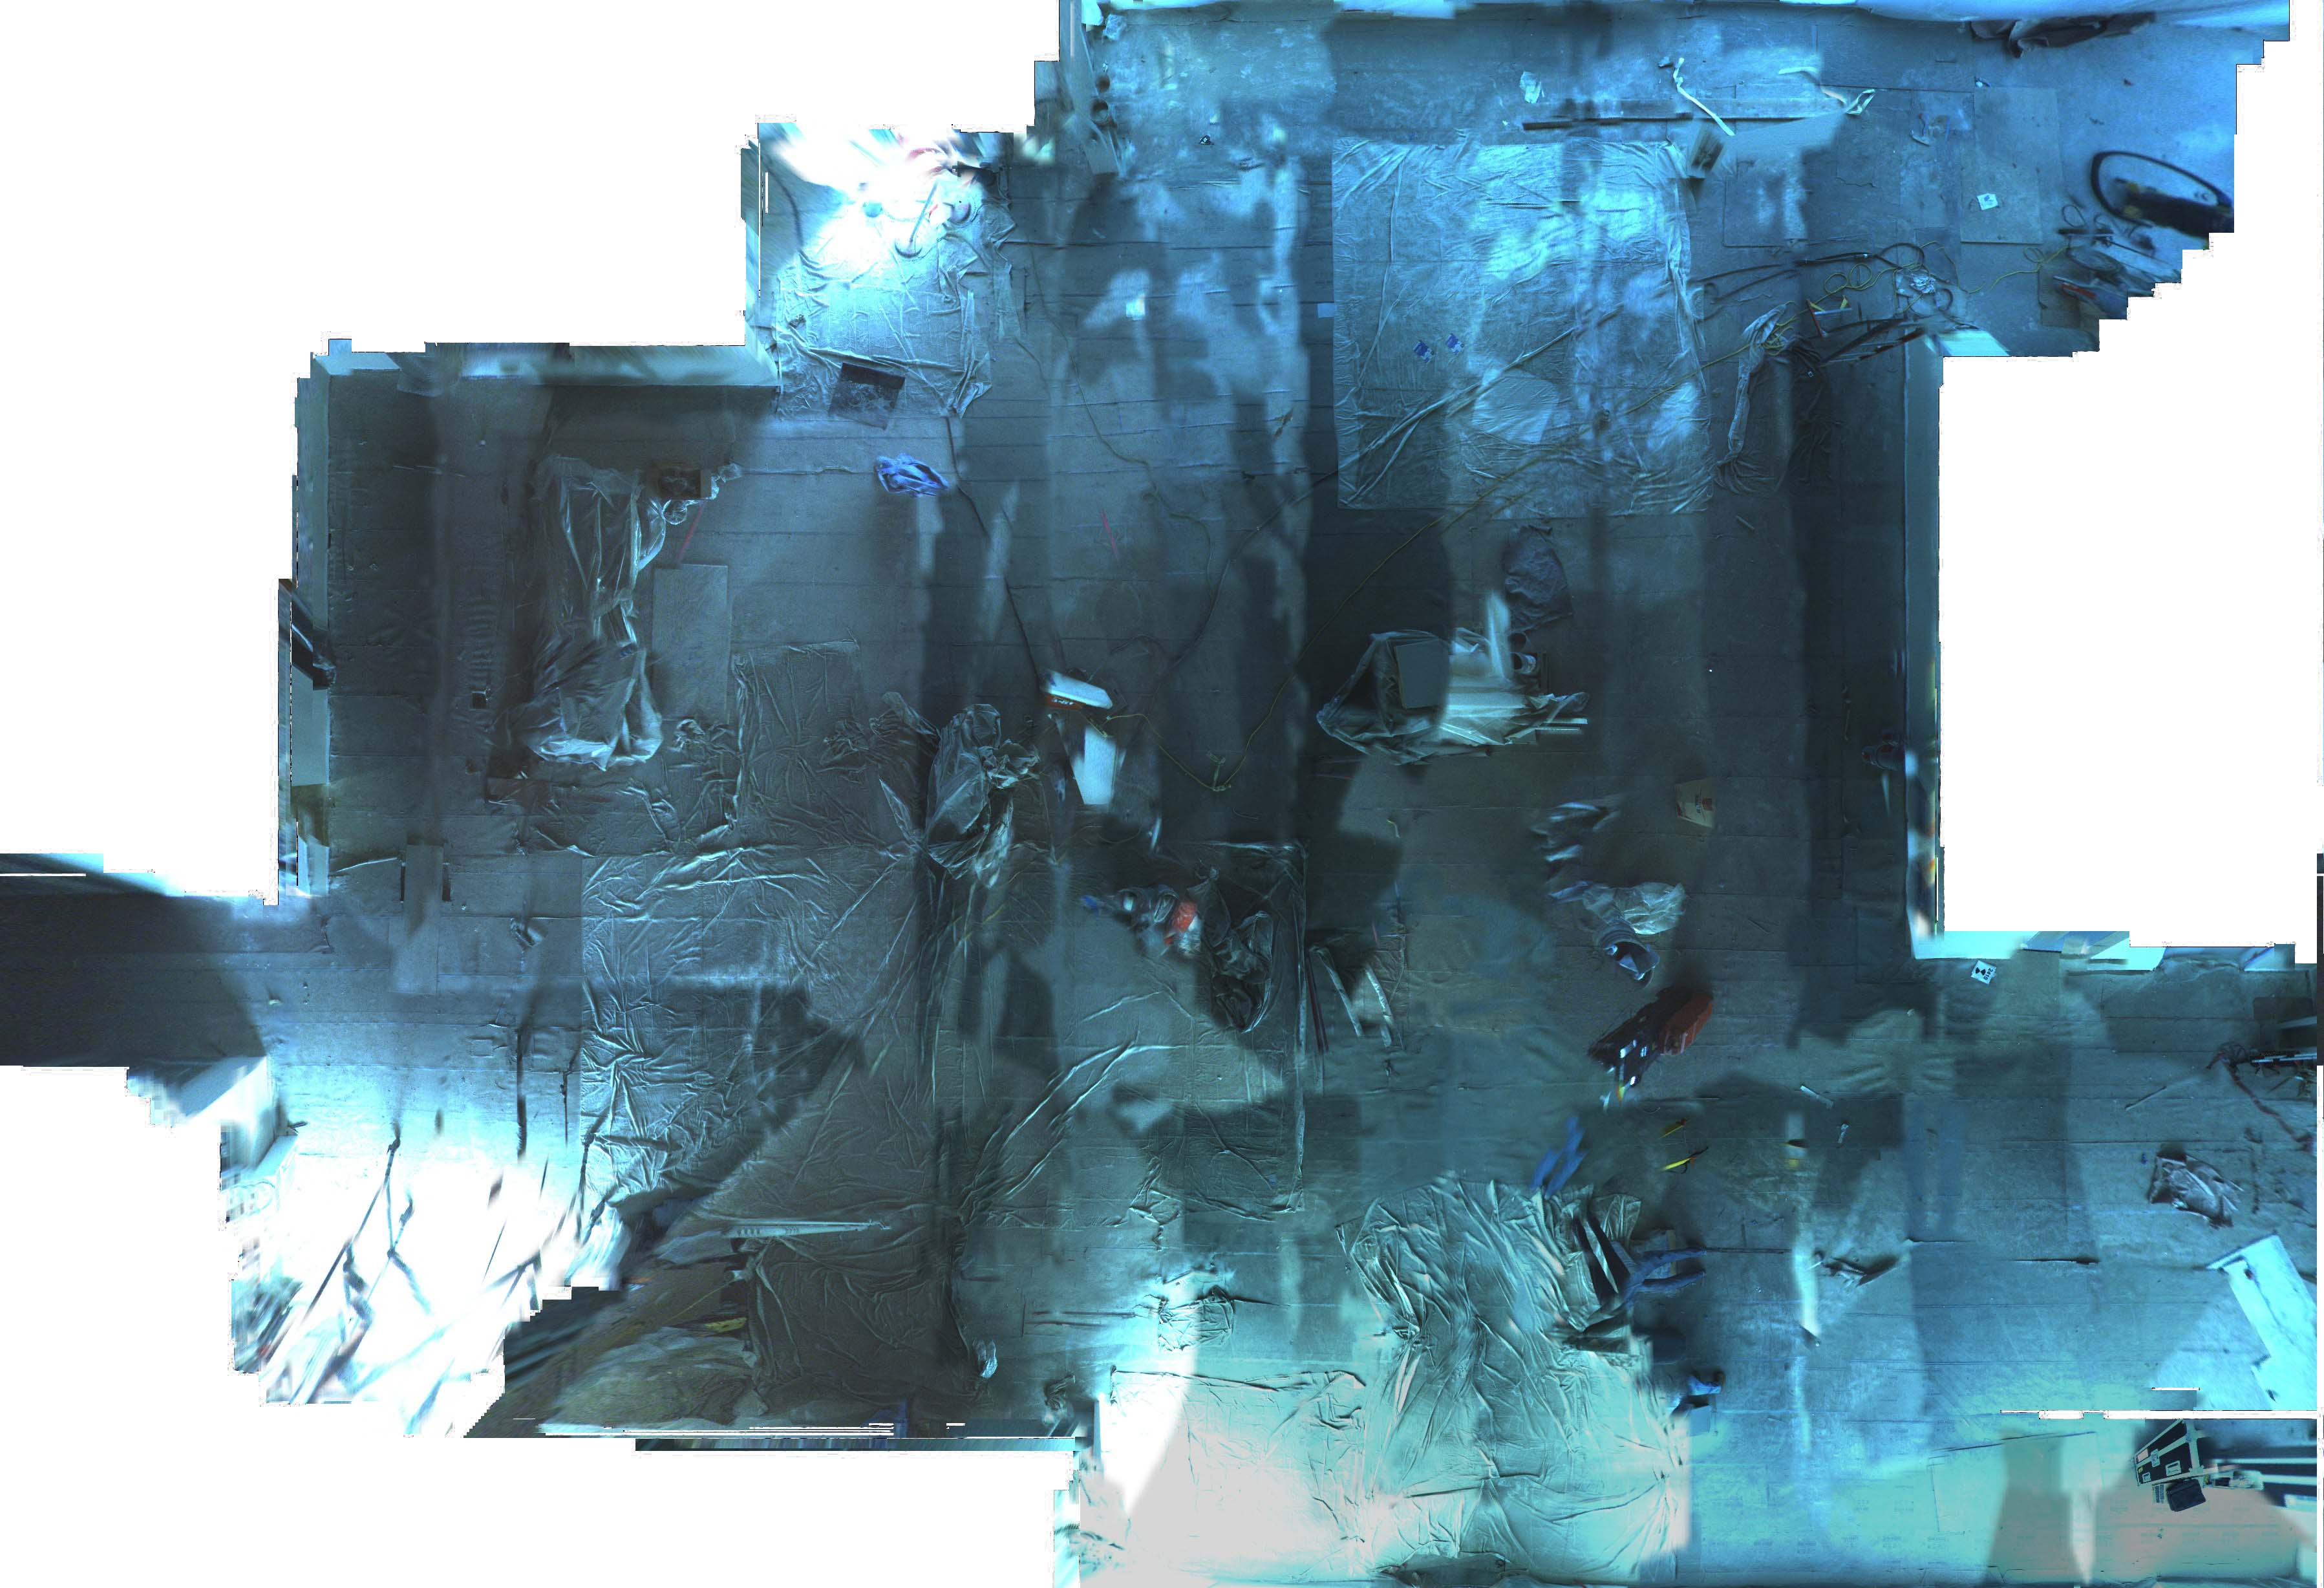
\includegraphics[width=3in]{pier15floor.jpg}
  }

  \centering{
    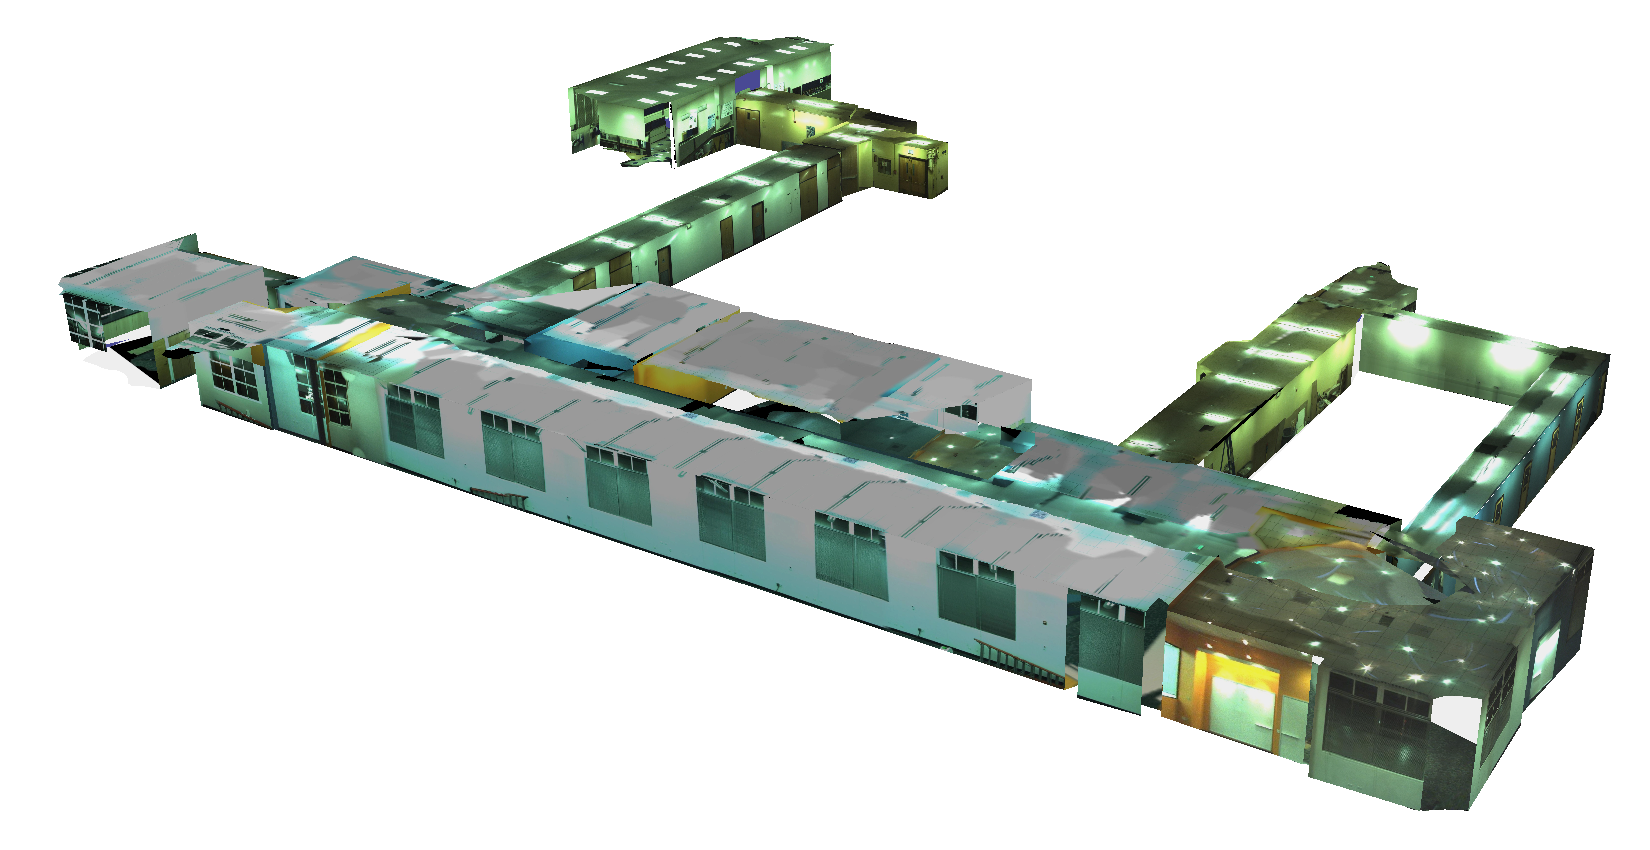
\includegraphics[width=1.9in]{fullmodel.png}
    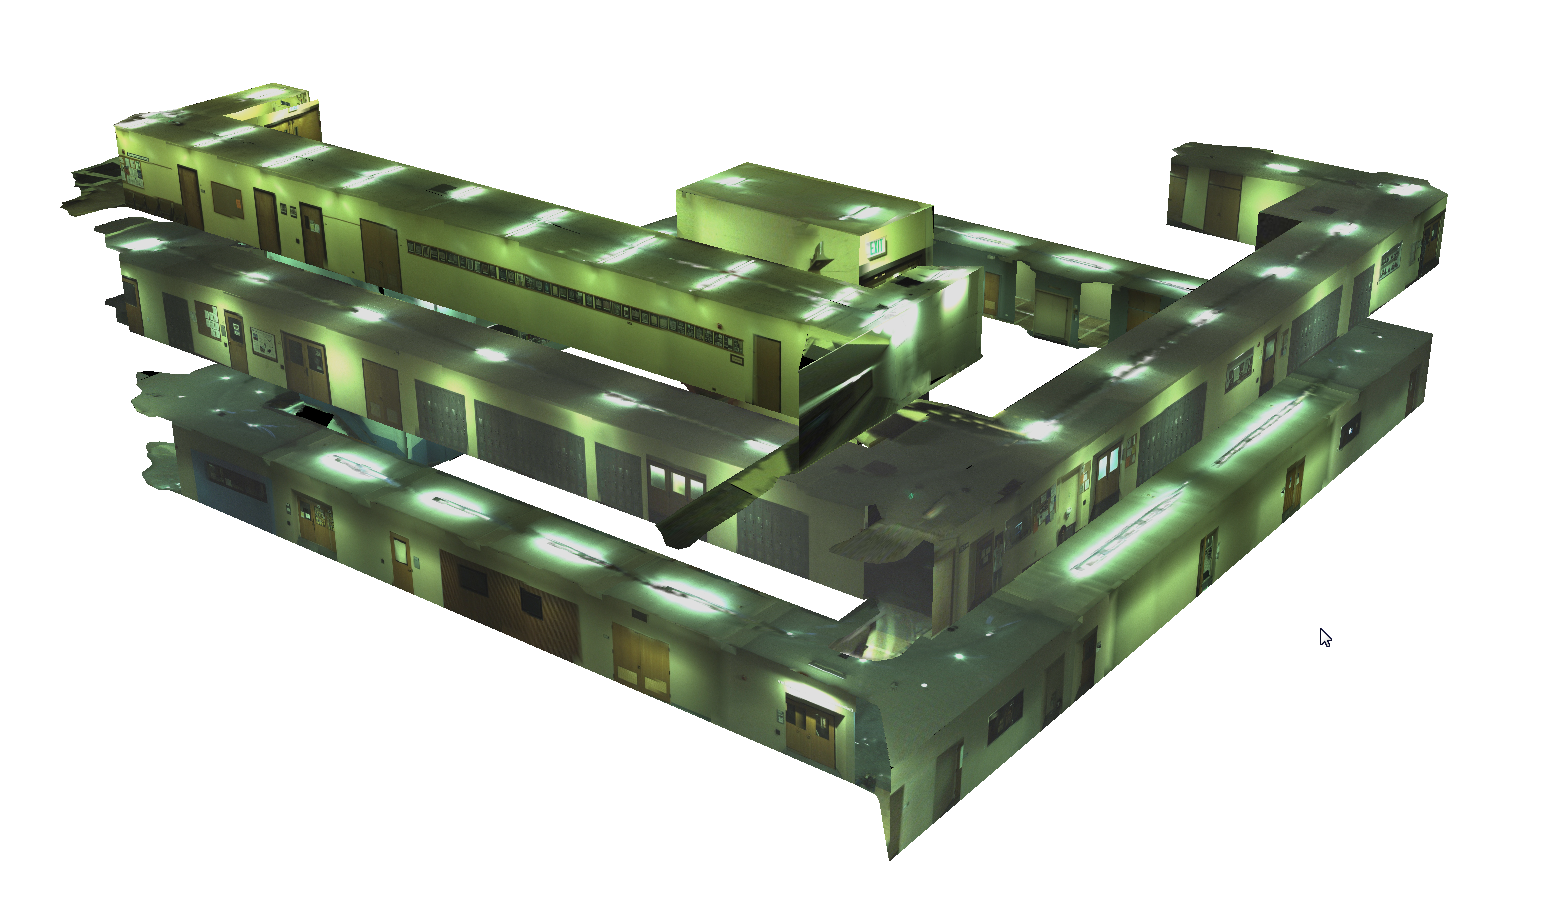
\includegraphics[width=1.9in]{threestoryfull2.png}
    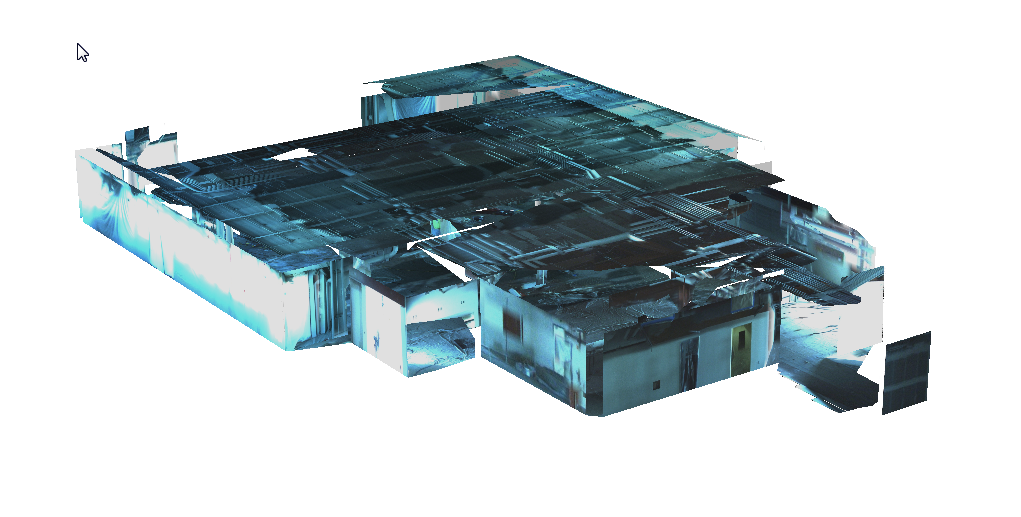
\includegraphics[width=1.9in]{pier15.png} \\
    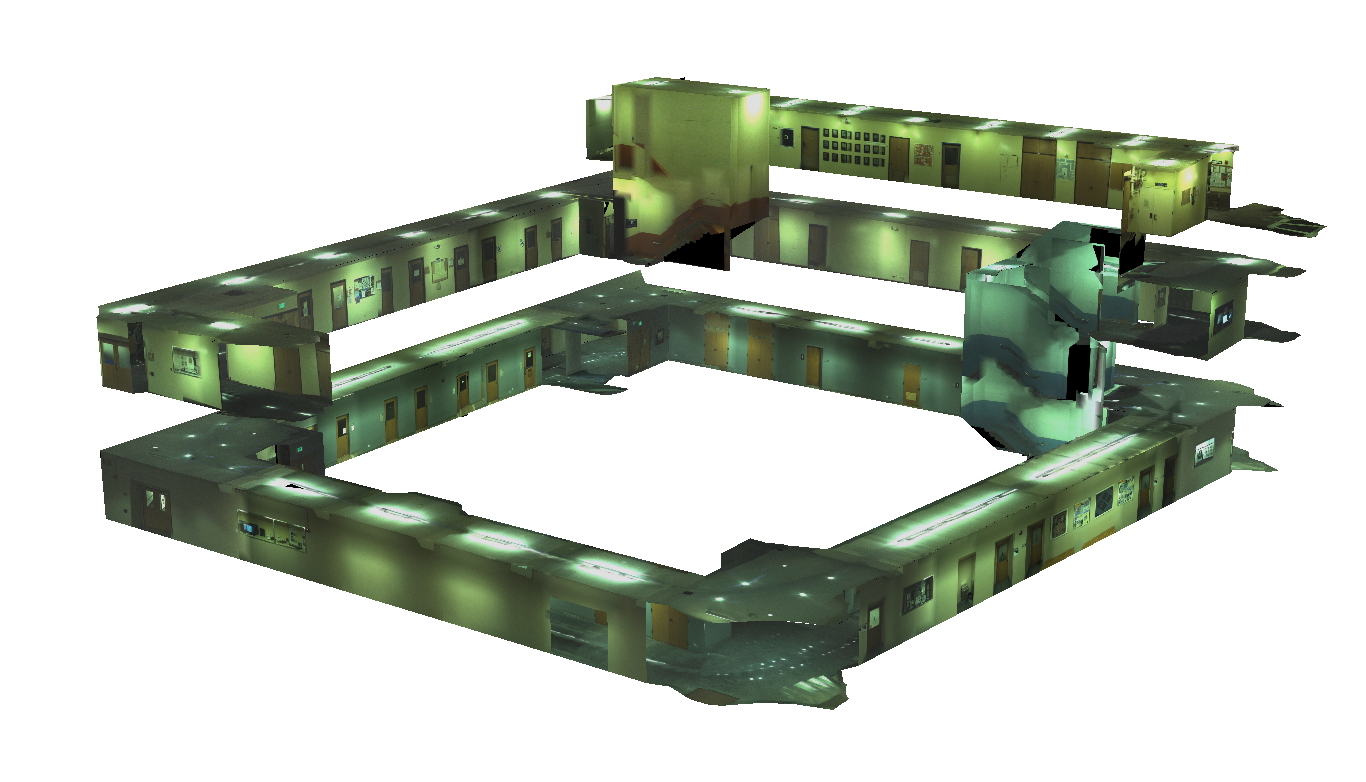
\includegraphics[width=6in]{threestoryfull.png}
  }

  \centering \subfloat[][]{ }
  \caption{Examples of our final texture mapping output for (a) walls,
    (b) ceilings, (c) floors, (d) full models.}
  \label{fig:results}
\end{figure}


%%%%%%%%%%%%%%%%%%%%%%%%%%%%%%%%%%%%%%%%%%%%%%%%%%%%%%%%%%%%%
%%%%% References %%%%%

\bibliography{report} %>>>> bibliography data in report.bib
\bibliographystyle{spiebib} %>>>> makes bibtex use spiebib.bst

\message{ !name(paper.tex) !offset(688) }

\end{document} 
